\chapter{Fundamentos teóricos}
\label{cap:fundamentos_teoricos}
Este capítulo se enfoca en analizar en profundidad los aspectos técnicos necesarios para llevar a cabo el desarrollo del CanSat.
Se incluye una comparativa entre los distintos microcontroladores y microcomputadores disponibles en el mercado, evaluando su precio, disponibilidad y adecuación a los requisitos técnicos del proyecto.
Además, se analizan los sensores y módulos de comunicación más comunes, así como los principales protocolos utilizados para la comunicación entre el microcontrolador y los sensores, como I2C y UART.
También se estudian distintas opciones para la retransmisión de vídeo en tiempo real desde el CanSat.
Por último, se exploran soluciones para la visualización de los datos a través de una interfaz web en tiempo real.


\section{Comparativa de microcontroladores y microcomputadores}
Uno de los componentes principales de un CanSat o de cualquier sistema embebido en general es su microcontrolador o microcomputador,
es el encargado de comunicarse con los sensores, procesar los datos y transmitirlo a través del módulo de comunicación,
también es el encargado de procesar el video y retransmitirlo en tiempo real(si el hardware lo permite).

Primero conviene aclarar la diferencia entre microcontrolador y microcomputador:
\begin{itemize}
    \item \textbf{Microcontrolador:} Circuito integrado que combina procesador, memoria y periféricos de entrada/salida en un solo chip.
    Está diseñado para realizar tareas específicas con bajo consumo energético y recursos limitados.
    Es común en aplicaciones como lectura de sensores, control de motores o gestión de comunicaciones básicas.
    Ejemplos comunes son Arduino Uno o ESP32
    \item \textbf{Microcomputador:} Sistema completo en una sola placa (Single-Board Computer) que integra procesador, memoria, almacenamiento y puertos de expansión.
    Es capaz de ejecutar sistemas operativos completos (como Linux) y realizar tareas más complejas, como procesamiento de imágenes, servidor web o interfaces gráficas.
    Un ejemplo típico es la Raspberry Pi Zero.
\end{itemize}

Actualmente, en el mercado se pueden encontrar varios de estos microcontroladores o microcomputadores de bajo coste, tamaño y peso reducido y bajo consumo.
En esta sección nos vamos a centrar en el análisis de tres de las opciones más populares:
\begin{itemize}

    \item \textbf{\cite{raspberrypi_zero2}:}
    La Raspberry Pi Zero 2 es un Single Board Computer de bajo costo lanzado en Reino Unido por la~\cite{raspberrypi_foundation},
    de toda la familia Raspberry Pi se ha elegido el modelo Zero 2 por ser el de tamaño más reducido pero con una potencia adecuada para el desarrollo de un proyecto como el CanSat.
    Las características más relevantes para este proyecto son:
    \begin{itemize}
        \item CPU Arm Cortex-A53 de cuatro núcleos y 64 bits a 1 GHz.
        \item SDRAM de 512 MB.
        \item LAN inalámbrica de 2,4 GHz 802.11 b/g/n.
        \item Bluetooth 4.2, Bluetooth Low Energy (BLE), antena integrada.
        \item Ranura para tarjeta microSD.
        \item Conector de cámara CSI-2.
        \item Cabecera GPIO de 40 pines para conexión de periféricos.
        \item 1 × SPI
        \item 2 × interfaces I²C
        \item 1 × UART
        \item Consumo típico de energía: entre 0.7\,W y 1.5\,W dependiendo de la carga de trabajo.
        \item Precio aproximado: 15–20€.
    \end{itemize}
    \begin{figure}[h]
        \centering
        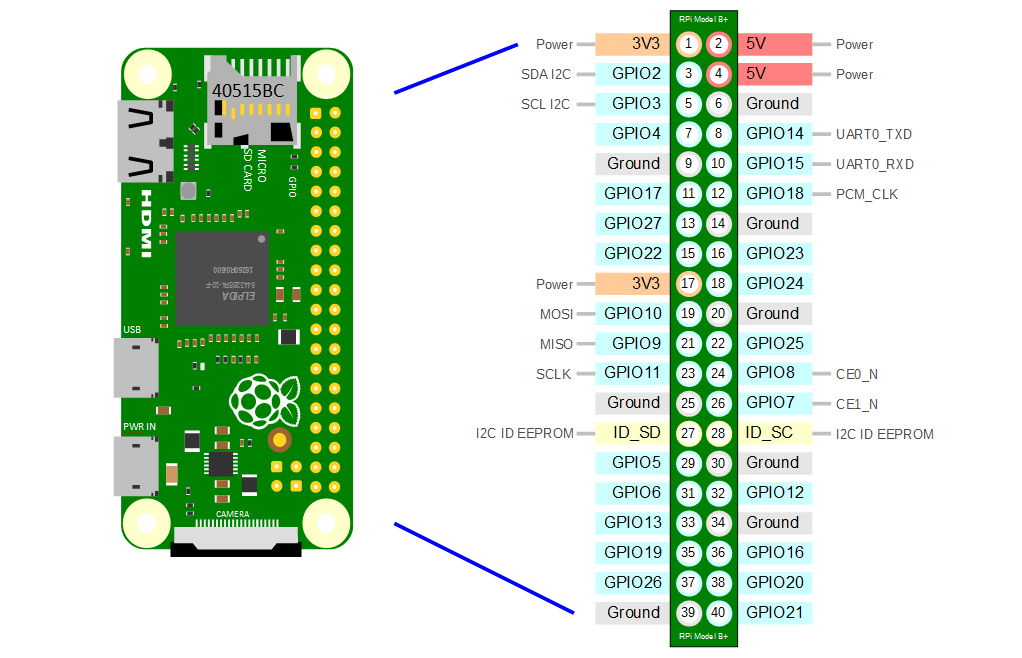
\includegraphics[width=0.8\textwidth]{Imagenes/Bitmap/pizero2gpio}
        \caption{Pines GPIO de la Raspberry Pi Zero 2}
        \label{fig:pizer2_gpio}
    \end{figure}
    Como se puede ver en las características la Raspberry Pi Zero 2 cumple con los requisitos necesarios para este proyecto,
    cuenta con un procesador y memoria adecuados, soporte para cámara (útil para la retransmisión de video en tiempo real), conectividad inalámbrica mediante WiFi
    y compatibilidad con los protocolos I\textsuperscript{2}C y UART mediante los pines GPIO necesarios para la conexión directa de sensores.

    \item \textbf{\cite{esp32}:}
    Es un microcontrolador de bajo coste desarrollado por Espressif Systems que combina bajo coste con buena capacidad de procesamiento y conectividad inalámbrica integrada,
    lo que lo convierte en una de las opciones más populares para proyectos embebidos, incluyendo CanSat.

    A diferencia de un microcomputador como la Raspberry Pi, el ESP32 no ejecuta un sistema operativo generalista,
    pero su bajo consumo energético y la integración de múltiples periféricos lo hacen convierten en muy buena opción cuando se busca eficiencia y simplicidad del sistema.

    Las características más relevantes para este proyecto son:
    \begin{itemize}
        \item CPU dual-core Tensilica Xtensa LX6 a 240\,MHz.
        \item 520\,KB de SRAM interna.
        \item Memoria flash externa: normalmente 4\,MB (dependiendo del modelo).
        \item Conectividad Wi-Fi 802.11 b/g/n.
        \item Bluetooth 4.2 y BLE.
        \item 4 × SPI
        \item 2 × interfaces I²C
        \item 3 × UART
        \item Hasta 34 pines GPIO (según versión del módulo).
        \item Consumo típico: entre 0.2\,W y 0.6\,W, dependiendo del modo de operación.
        \item Precio aproximado: 4–8€~\cite{esp32}.
    \end{itemize}
    \begin{figure}[h]
        \centering
        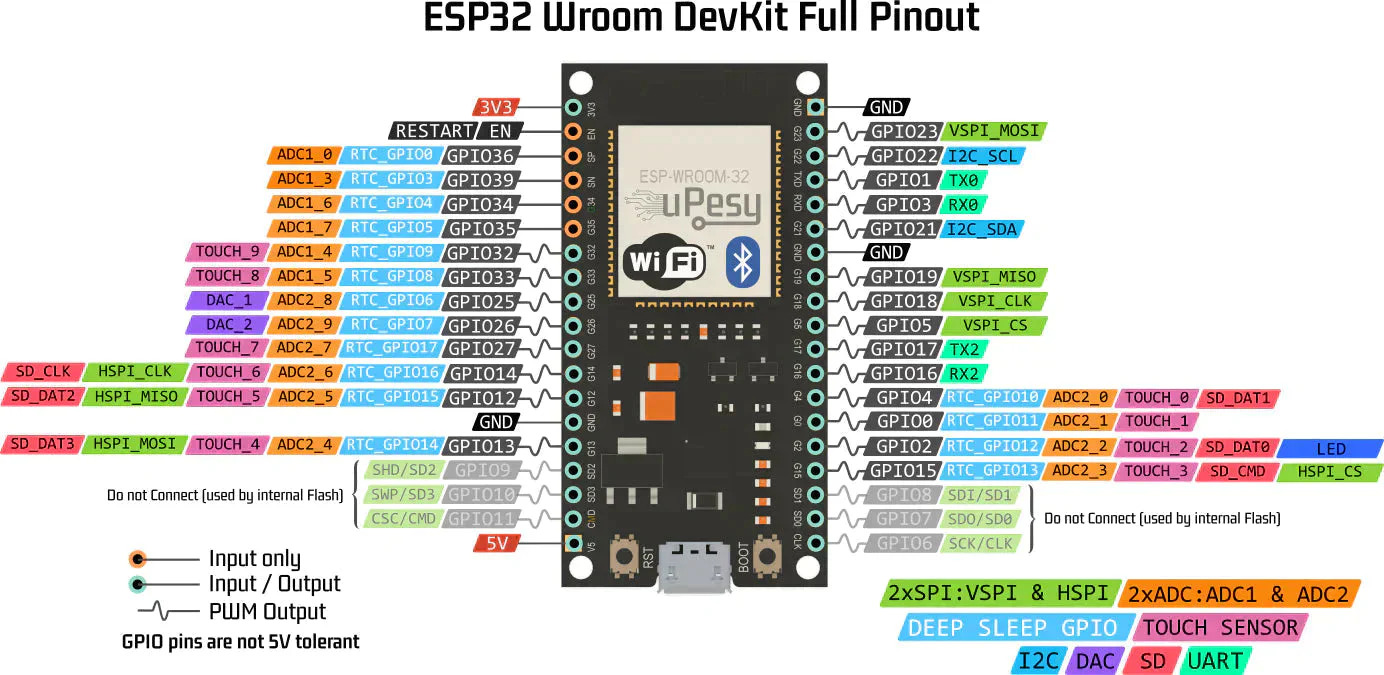
\includegraphics[width=0.8\textwidth]{Imagenes/Bitmap/esp32gpio}
        \caption{Pines GPIO de la Raspberry Pi Zero 2}
        \label{fig:esp32gpio}
    \end{figure}

    Gracias a su bajo consumo, potencia y multiples conexiones, el ESP32 permite integrar sensores fácilmente a través de interfaces estándar y puede encargarse tanto de la adquisición como de la transmisión de datos por radio o Wi-Fi.
    Además, su bajo consumo lo hace especialmente adecuado para sistemas alimentados por batería en entornos con restricciones energéticas.
    También existen variantes como el ESP32-CAM que integran una cámara de tipo OV2640, lo que permite capturar imágenes y transmitir video mediante Wi-Fi
    aunque con un rendimiento y resolución inferior a la de Raspberry Pi.

    \item \textbf{\cite{arduino_nano}:}
    Es un microcontrolador compacto de bajo coste basado en el chip ATmega328P, es el más utilizado en entornos educativos gracias a su simplicidad,
    por lo que cuenta con una amplia comunidad detrás y desarrollo de librerias.
    A diferencia de la Raspberry Pi Zero 2 o el ESP32, el Arduino Nano no cuenta con conectividad inalámbrica ni capacidad de procesamiento avanzada,
    pero es suficiente para gestionar sensores básicos y transmitir datos mediante un módulo externo de radio.

    Las características más relevantes para este proyecto son:
    \begin{itemize}
        \item Microcontrolador ATmega328P.
        \item Frecuencia de reloj: 16\,MHz.
        \item Memoria flash: 32\,KB (2\,KB utilizados por el bootloader).
        \item SRAM: 2\,KB.
        \item EEPROM: 1\,KB.
        \item 22 pines GPIO (14 digitales, 8 analógicos).
        \item 1 × interfaz I²C.
        \item 1 × UART.
        \item 1 × SPI.
        \item Consumo típico: entre 0.05\,W y 0.2\,W.
        \item Precio aproximado: 27€ en la web oficial.
    \end{itemize}

    \begin{figure}[h]
        \centering
        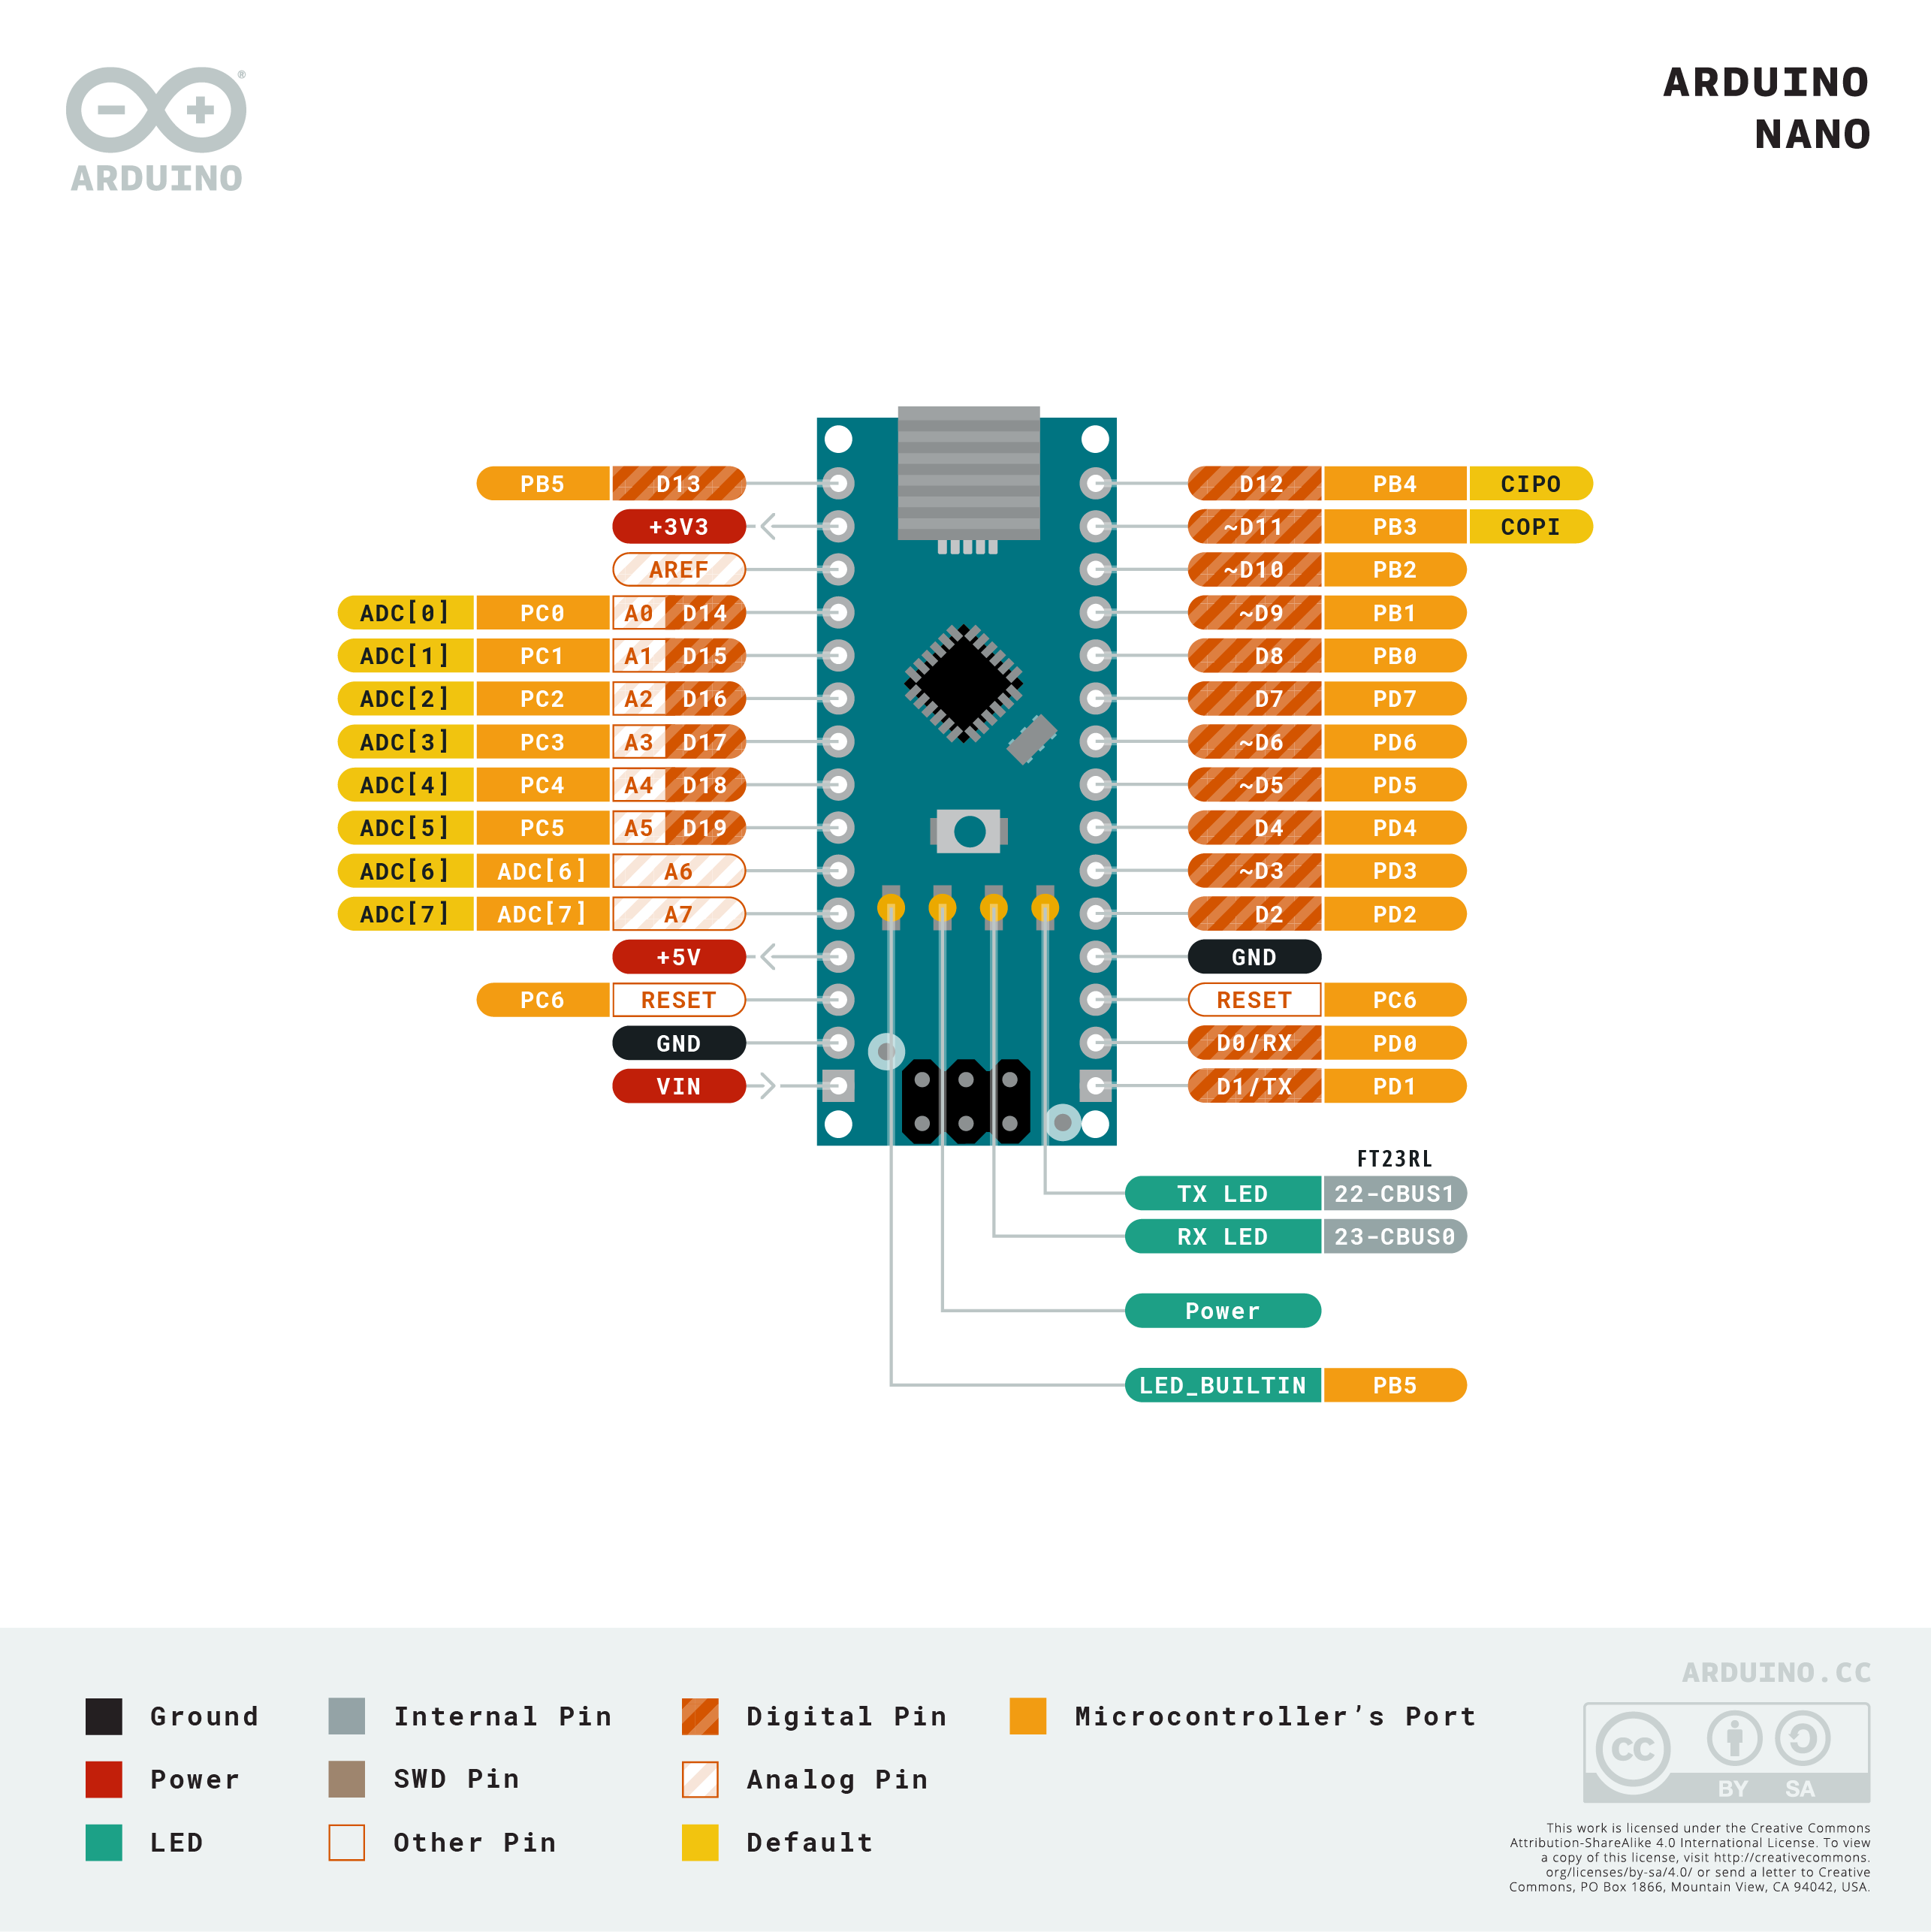
\includegraphics[width=0.7\textwidth]{Imagenes/Bitmap/arduinoNanogpio}
        \caption{Distribución de pines en el Arduino Nano}
        \label{fig:arduino_nano_gpio}
    \end{figure}

    Aunque no tiene las capacidades de procesamiento de una Raspberry Pi ni la conectividad integrada del ESP32, el Arduino Nano puede ser una solución válida para CanSat muy simples,
    en los que se priorice el consumo mínimo y no se necesiten funcionalidades avanzadas como WiFi o procesamiento de vídeo, sin embargo, al no tener soporte para cámaras,
    no cumple con los requisitos técnicos necesarios para este proyecto.

\end{itemize}


\section{Protocolos de comunicación: I2C y UART}


\section{Transmisión de datos mediante LoRa}


\section{Sensores embarcados: presión, orientación y GPS}


\section{Captura y transmisión de vídeo en tiempo real}


\section{Visualización de datos en tiempo real: arquitecturas orientadas a eventos}


\section{Modelado 3D de orientación con cuaterniones}